%++++++++++++++++++++++++++++++++++++++++
% Don't modify this section unless you know what you're doing!
\documentclass[letterpaper,12pt]{article}
\usepackage{tabularx} % extra features for tabular environment
\usepackage{amsmath}  % improve math presentation
\usepackage{graphicx} % takes care of graphic including machinery
\usepackage[margin=1in,letterpaper]{geometry} % decreases margins
\usepackage{cite} % takes care of citations
\usepackage[final]{hyperref} % adds hyper links inside the generated pdf file
\usepackage{pgfplotstable, booktabs}
\usepackage{placeins}
\usepackage{tabularray}
\usepackage{titlesec}
\usepackage{fancyhdr}
\usepackage{empheq}
\usepackage{amssymb}
\usepackage{sectsty}
\usepackage{tcolorbox}
\usepackage{listings}
\usepackage{xcolor}
\usepackage{parskip}
\usepackage{cancel}
\usepackage{enumitem}
\usepackage{amsmath}
\usepackage{mathrsfs}
\usepackage{physics}
\usepackage{subcaption}
\usepackage{pdfpages}
\usepackage{amsthm} 
\usepackage{float}

\definecolor{codegreen}{rgb}{0,0.6,0}
\definecolor{codegray}{rgb}{0.5,0.5,0.5}
\definecolor{codepurple}{rgb}{0.58,0,0.82}

\lstdefinestyle{mystyle}{
    commentstyle=\color{codegreen},
    keywordstyle=\color{codepurple},
    numberstyle=\tiny\color{codegray},
    stringstyle=\color{codegreen},
    basicstyle=\ttfamily\small,
    breakatwhitespace=false,         
    breaklines=true,                 
    captionpos=b,                    
    keepspaces=true,                                                     
    showspaces=false,                
    showstringspaces=false,
    showtabs=false,                  
    tabsize=4
}

\lstset{style=mystyle}
  
\newcommand*\widefbox[1]{\fbox{\hspace{0em}#1\hspace{0em}}}
%define a divergence command which does \text{div}
\DeclareMathOperator{\Div}{Div}


\pagestyle{fancy}
\fancyhf{} % Clear all header and footer fields
\fancyhead[L]{MEC E 539}
%\fancyhead[C]{Center Header} 
\fancyhead[C]{Assignment 2}
\fancyhead[R]{Alex Diep}

\fancyfoot[C]{\thepage}

\pgfplotsset{compat=1.18} 
\titleformat*{\section}{\Large\bfseries}
\titleformat*{\subsection}{\large\bfseries}

\renewcommand{\thesection}{Question \arabic{section}}
\renewcommand{\thesubsection}{(\alph{subsection})}
\renewcommand*{\arraystretch}{1.5}

\hypersetup{
	colorlinks=true,       % false: boxed links; true: colored links
	linkcolor=blue,        % color of internal links
	citecolor=blue,        % color of links to bibliography
	filecolor=magenta,     % color of file links
	urlcolor=blue         
}
%++++++++++++++++++++++++++++++++++++++++
\begin{document}
% \begin{titlepage}
%     \centering
%     \vspace*{2cm} % Adjust vertical spacing
    
%     % Title
%     \Huge {MEC E 301 \\Lab 1: Dimensional Measurement} \\
%     \vspace{1cm} % Adjust vertical spacing
    
%     % Author
%     \Large by: Alex Diep \\
%     \vspace{1cm} % Adjust vertical spacing

%     % Date
%     \Large Date: September 19, 2023 \\ % or manually specify a date
%     \vspace{4cm} % Adjust vertical spacing

%     % CCID and Student ID in smtaller font
%     \normalsize CCID: abdiep \\
%     \normalsize Student ID: 1664334 \\ 
%     \normalsize Section: D21 \\
    
%     \vfill % Fill vertical space
    
%     % Additional content (e.g., university logo or other information)
    
% \end{titlepage}

% Consider laminar flow between two parallel plates (Fig. 1). Plates extend infinitely in x and
% z directions. The following assumptions are made:
% • the flow is at steady state (no time dependency)
% • the fluid is incompressible, ideal and Newtonian
% • the temperature of the bottom plate is Tb and the upper plate is at temperature Tu
% • vy = vz = 0
% • vx = vx(y), T = T(y)
% Figure 1: Problem statement: fluid flow between two parallel plates. The bottom plate is
% fixed, the upper plate is moving horizontally with velocity uw. The fluid is incompressible
% and Newtonian.


\section{}
\textit{Write down the full set of governing equations (continuity, momentum and energy).}

\begin{figure}[h]
    \centering
    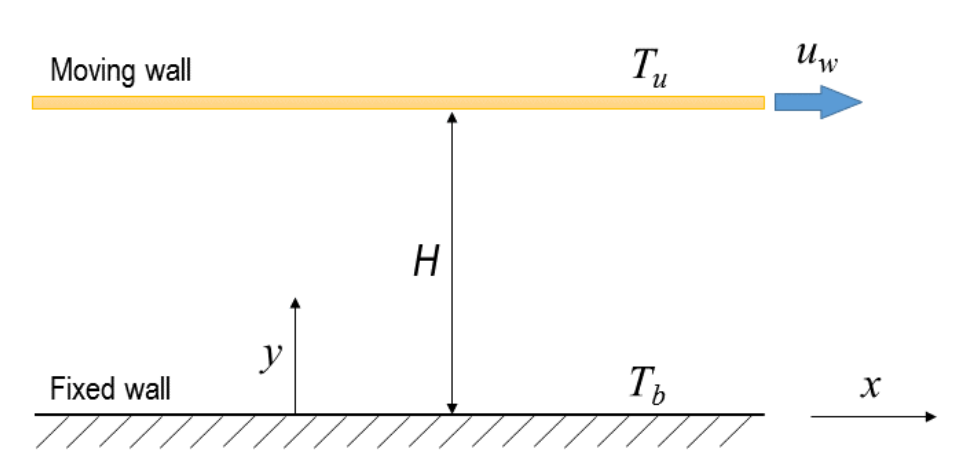
\includegraphics[width=0.5\textwidth]{Questions/Figures/Q1 diagram.png}
    \caption{Fluid flow betweeen parallel plates. The bottom plate is fixed, the upper plate is moving horizontally with velocity $u_w$. THe fluid is incompressible and Newtonian.}
    \label{fig:Q1 diagram}
\end{figure}

\subsection*{Solution}
We first begin with continuity, 
\begin{align*}
    \Aboxed{\frac{\partial \rho}{\partial t} + \vec{u} \cdot \nabla \rho + \rho (\nabla \cdot \vec{u}) &= 0}
\end{align*}
then, the momentum equation,
\begin{align*}
    \Aboxed{\frac{\partial}{\partial t} (\rho u_i) + \frac{\partial}{\partial x_j} (\rho u_i u_j) &= -\frac{\partial P}{\partial x_i} + \frac{\partial}{\partial x_j} \left[ \mu \left( \frac{\partial u_i}{\partial x_j} + \frac{\partial u_j}{\partial x_i} \right) \right] - \frac{\partial}{\partial x_i} \left(\frac{2}{3} \mu \frac{\partial u_k}{\partial x_k} \right) + \rho b_i}
\end{align*}
lastly, the energy equation,
\begin{align*}
    \Aboxed{\rho C_p \left(\frac{\partial T}{\partial t} + \vec{v} \cdot \nabla T \right) &= k \nabla^2 T + \frac{\mu}{2} \Phi^2}
\end{align*}
where $\Phi_{i, j} = \left( \frac{\partial u_i}{\partial x_j} + \frac{\partial u_j}{\partial x_i} \right)$.



\section{}
\textit{Provide a clean vector plot of the flow velocity that clearly illustrates the mixing of two
streams of air. Particularly, what do these vector results indicate about the flow physics?
Use screenshots and other illustrations to support your statement.}

\subsection*{Solution}
\begin{figure}[h]
    \centering
    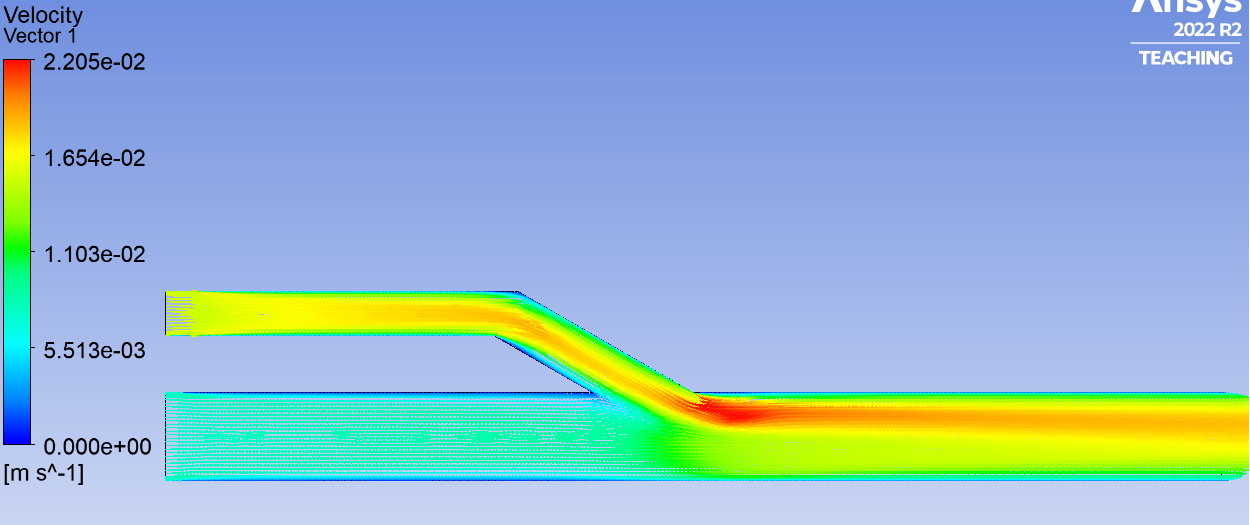
\includegraphics[width=0.8\textwidth]{Questions/Figures/velocity vector.png}
    \caption{Vector field plot of the flow velocity}
    \label{fig:contour}
\end{figure}

The velocity plot shows much of the same information as the contour plot. The plot clearly illustrates the mixing of two streams of air. The plot indicates that the higher velocity flow `pushes' down the lower velocity field. As the flow continues, the stream seems to `mix' the velocities to an average velocity as it approaches the outlet.

For both the upper and lower flows, a boundary layer can be seen developing starting from the inlet. The boundary layer is more pronounced for the upper flow.

Also, the velocity of the upper stream increases around the corner where the flows mix.
\section{}
\textit{Solve the simplified momentum equation.}

\subsection*{Solution}
Using no-slip boundary conditions, the boundary conditions are 
\begin{align*}
    u_x(0) &= 0 \\
    u_x(H) &= u_w
\end{align*}

The simplified momentum equation in the $x$-direction is given by
\begin{align*}
    \frac{\partial^2 u_x}{\partial y^2} &= 0
\end{align*}
which has the general solution
\begin{align*}
    u_x(y) &= A y + B
\end{align*}
where $A$ and $B$ are constants. Applying the boundary conditions, we find
\begin{align*}
    u_x(0) &= B = 0 \\
    u_x(H) &= A H = u_w
\end{align*}
which gives
\begin{align*}
    u_x(y) &= \frac{u_w}{H} y
\end{align*}
This linear profile is also known as Couette flow. Next, the simplified momentum equation in the $y$-direction is given by
\begin{align*}
    \frac{\partial P}{\partial y} &= 0
\end{align*}
which has the general solution
\begin{align*}
    P &= C(z)
\end{align*}
where $C(z)$ is a function of $z$. Lastly, the simplified momentum equation in the $z$-direction is given by
\begin{align*}
    \frac{\partial P}{\partial z} &= -\rho g
\end{align*}
which has the general solution
\begin{align*}
    P(z) &= -\rho g z + D
\end{align*}
where $D$ is a constant.

So in summary, 
\begin{empheq}[box=\fbox]{align*}
    \vec{u} &= \left[\frac{u_w}{H} y\right] \hat{i} \\
    P &= -\rho g z + D
\end{empheq}
\section{}
% \textit{Substitute approximations obtained in Questions 2 and 3 back
% into equation derived in Question 1. Rearrange the obtained equation into a form}
\textit{Substitute approximations obtained in Questions 2 and 3 back into equation derived in Question 1. Rearrange the obtained equation into a form that can be used to solve for $\hat{T}_P$.}
\begin{align*}
    a_P T_P &= a_W T_W + a_E T_E 
\end{align*}
\textit{and identify coefficients $a_P$, $a_W$, $a_E$, $q_{T}^{u}$, and $q_{T}^{P}$.} \\

Substituting back into the equation derived in Question 1,
\begin{align*}
    \hat{T}_P - \hat{T}_W &= \frac{1}{\text{Pe}} \left(\frac{\hat{T}_E - 2\hat{T}_P + \hat{T}_W}{\Delta x}\right) 
\end{align*}
Rearranging,
\begin{align*}
    %\left[\frac{2}{\text{Pe}\Delta x} + 1\right]\hat{T}_P &= \left[\frac{1}{\text{Pe}\Delta x} + 1\right]\hat{T}_W + \left[\frac{1}{\text{Pe}\Delta x}\right]\hat{T}_E + [0] q_{T}^{u} 
    \underbrace{\left[\frac{2}{\text{Pe}\Delta x} + 1\right]}_{a_P}\hat{T}_P &= \underbrace{\left[\frac{1}{\text{Pe}\Delta x} + 1\right]}_{a_W}\hat{T}_W + \underbrace{\left[\frac{1}{\text{Pe}\Delta x}\right]}_{a_E}\hat{T}_E + [0] q_{T}^{u} + [0] q_{T}^{P}
\end{align*}
\section{}
\textit{Solve the simplified energy equation.}
\subsection*{Solution}
The simplified energy equation is given by
\begin{equation*}
    \frac{\partial^2 T}{\partial y^2} = -\frac{\mu}{k} \left(\frac{u_w}{H}\right)^2
\end{equation*}
Integrating twice with respect to $y$,
\begin{align*}
    \frac{\partial T}{\partial y} &= -\frac{\mu}{k} \left(\frac{u_w}{H}\right)^2 y + C_1 \\
    T &= -\frac{\mu}{2k} \left(\frac{u_w}{H}\right)^2 y^2 + C_1 y + C_2
\end{align*}
Applying the boundary conditions $T(0) = T_b$ and $T(H) = T_u$,
\begin{align*}
    T_b &= C_2 \\
    T_u &= -\frac{\mu}{2k} \left(\frac{u_w}{H}\right)^2 H^2 + C_1 H + C_2 \implies C_1 = \frac{T_u - T_b + \frac{\mu}{2k} \left(\frac{u_w}{H}\right)^2 H^2}{H}
\end{align*}
Thus, the temperature profile is given by
\begin{empheq}[box=\fbox]{align*}
    T(y) &= -\frac{\mu}{2k} \left(\frac{u_w}{H}\right)^2 y^2 + \left(\frac{T_u - T_b + \frac{\mu}{2k} \left(\frac{u_w}{H}\right)^2 H^2}{H}\right) y + T_b
\end{empheq}

\section{}
\textit{Rearrange the obtained equation into a general form}
\[
    a_P T_P = a_W T_W + a_E T_E + q_{T}^{u}
\]
\textit{and identify coefficients $a_P$, $a_W$, $a_E$, $q_{T}^{u}$, and $q_{P}^{T}$.}\\

From Q5, the equation obtained is,
\begin{align*}
    \hat{T}_E - \hat{T}_P &= \frac{1}{\text{Pe}} \left(\frac{\hat{T}_E + 2 \hat{T}_A - 3 \hat{T}_P}{\Delta x}\right) 
\end{align*}
Expanding the equation,
\begin{align*}
    \underbrace{\left[\frac{3}{\text{Pe} \Delta x} -1\right]}_{a_P}\hat{T}_P &= \underbrace{[0]}_{a_W}\hat{T}_W + \underbrace{\left[\frac{1}{\text{Pe} \Delta x} -1\right]}_{a_E}\hat{T}_E + \underbrace{\frac{2}{\text{Pe} \Delta x} \hat{T}_A}_{q_{T}^{u}} + \underbrace{0}_{q_{P}^{T}}
\end{align*}
\section{}
\textit{Integrate eq. (2) over boundary control volume 5 and approximate the convective term using upwind scheme. Use central difference scheme for the approximation of the diffusive term. Assume constant cross section value $S = 1$.} \\

Integrating Eq. 2, but over control volume 5,
\begin{align*}
    \int_{\Delta x} \frac{d \hat{T}}{dx} S dx &= \int_{\Delta x} \frac{d}{dx}\left(\frac{1}{\text{Pe}} \frac{d \hat{T}}{dx}\right) S dx \\
    \hat{T} \bigg|_{w}^{B} &= \left(\frac{1}{\text{Pe}} \frac{d \hat{T}}{dx}\right) \bigg|_{w}^{B}
\end{align*}
Then,
\begin{align*}
    \Aboxed{\underbrace{\hat{T}_w - \hat{T}_B}_{\text{Convective}} &= \underbrace{\frac{1}{\text{Pe}} \left[\frac{d \hat{T}}{dx}\right]_w - \frac{1}{\text{Pe}} \left[\frac{d \hat{T}}{dx}\right]_B}_{\text{Diffusive}}}
\end{align*}
For the convective term, upwind scheme is used,
\begin{align*}
    \hat{T}_B &= \hat{T}_P \\
    \hat{T}_w &= \hat{T}_W 
\end{align*}
Then,
\begin{align*}
    \text{Convective} &= \hat{T}_w - \hat{T}_B \\
    &= \hat{T}_W - \hat{T}_P
\end{align*}
For the diffusive term, a central difference scheme is used,
\begin{align*}
    \left[\frac{d \hat{T}}{dx}\right]_w &= \frac{\hat{T}_P - \hat{T}_W}{\Delta x} \\
    \left[\frac{d \hat{T}}{dx}\right]_B &= \frac{\hat{T}_B - \hat{T}_P}{\Delta x/2}
\end{align*}
Substituting back into the equation derived,
\begin{align*}
    \Aboxed{\hat{T}_W - \hat{T}_P &= \frac{1}{\text{Pe}} \left(\frac{3 \hat{T}_P - \hat{T}_W - 2 \hat{T}_B}{\Delta x}\right)} 
\end{align*}
\section{}
% Rearrange the obtained equation into a general form
% aP TP = aW TW + aETE + q
% u
% T
% and identify coefficients aP , aW , aE, q
% u
% T
% , and q
% P
% T
% .

% \section{}
% \textit{Rearrange the obtained equation into a general form}
% \[
%     a_P T_P = a_W T_W + a_E T_E + q_{T}^{u}
% \]
% \textit{and identify coefficients $a_P$, $a_W$, $a_E$, $q_{T}^{u}$, and $q_{P}^{T}$.}\\

% From Q5, the equation obtained is,
% \begin{align*}
%     \hat{T}_E - \hat{T}_P &= \frac{1}{\text{Pe}} \left(\frac{\hat{T}_E + 2 \hat{T}_A - 3 \hat{T}_P}{\Delta x}\right) 
% \end{align*}
% Expanding the equation,
% \begin{align*}
%     %\left[\frac{3}{\text{Pe} \Delta x} -1\right]\hat{T}_P &= \left[\frac{1}{\text{Pe} \Delta x} -1\right]\hat{T}_E + \frac{2}{\text{Pe} \Delta x}\hat{T}_A
%     \underbrace{\left[\frac{3}{\text{Pe} \Delta x} -1\right]}_{a_P}\hat{T}_P &= \underbrace{[0]}_{a_W}\hat{T}_W + \underbrace{\left[\frac{1}{\text{Pe} \Delta x} -1\right]}_{a_E}\hat{T}_E + \underbrace{\frac{2}{\text{Pe} \Delta x}}_{q_{T}^{u}} \hat{T}_A + \underbrace{0}_{q_{P}^{T}}
% \end{align*}
% \section{}
% \textit{Integrate eq. (2) over boundary control volume 5 and approximate the convective term using upwind scheme. Use central difference scheme for the approximation of the diffusive term. Assume constant cross section value $S = 1$.} \\

% Integrating Eq. 2, but over control volume 5,
% \begin{align*}
%     \int_{\Delta x} \frac{d \hat{T}}{dx} S dx &= \int_{\Delta x} \frac{d}{dx}\left(\frac{1}{\text{Pe}} \frac{d \hat{T}}{dx}\right) S dx \\
%     \hat{T} \bigg|_{w}^{B} &= \left(\frac{1}{\text{Pe}} \frac{d \hat{T}}{dx}\right) \bigg|_{w}^{B}
% \end{align*}
% Then,
% \begin{align*}
%     \Aboxed{\underbrace{\hat{T}_w - \hat{T}_B}_{\text{Convective}} &= \underbrace{\frac{1}{\text{Pe}} \left[\frac{d \hat{T}}{dx}\right]_w - \frac{1}{\text{Pe}} \left[\frac{d \hat{T}}{dx}\right]_B}_{\text{Diffusive}}}
% \end{align*}
% For the convective term, upwind scheme is used,
% \begin{align*}
%     \hat{T}_B &= \hat{T}_P \\
%     \hat{T}_w &= \hat{T}_W 
% \end{align*}
% Then,
% \begin{align*}
%     \text{Convective} &= \hat{T}_w - \hat{T}_B \\
%     &= \hat{T}_W - \hat{T}_P
% \end{align*}
% For the diffusive term, a central difference scheme is used,
% \begin{align*}
%     \left[\frac{d \hat{T}}{dx}\right]_w &= \frac{\hat{T}_P - \hat{T}_W}{\Delta x} \\
%     \left[\frac{d \hat{T}}{dx}\right]_B &= \frac{\hat{T}_B - \hat{T}_P}{\Delta x/2}
% \end{align*}
% Substituting back into the equation derived,
% \begin{align*}
%     \Aboxed{\hat{T}_W - \hat{T}_P &= \frac{1}{\text{Pe}} \left(\frac{3 \hat{T}_P - \hat{T}_W - 2 \hat{T}_B}{\Delta x}\right)} 
% \end{align*}

\textit{Rearrange the obtained equation into a general form}
\[
    a_P T_P = a_W T_W + a_E T_E + q_{T}^{u}
\]
\textit{and identify coefficients $a_P$, $a_W$, $a_E$, $q_{T}^{u}$, and $q_{P}^{T}$.}\\

From Q7, the equation obtained is,
\begin{align*}
    \hat{T}_W - \hat{T}_P &= \frac{1}{\text{Pe}} \left(\frac{3 \hat{T}_P - \hat{T}_W - 2 \hat{T}_B}{\Delta x}\right)
\end{align*}
Expanding the equation,
\begin{align*}
    \underbrace{\left[\frac{-3}{\text{Pe} \Delta x} -1\right]}_{a_P}\hat{T}_P &= \underbrace{\left[\frac{-1}{\text{Pe} \Delta x} -1\right]}_{a_W}\hat{T}_W + \underbrace{[0]}_{a_E}\hat{T}_E + \underbrace{\frac{-2}{\text{Pe} \Delta x} \hat{T}_B}_{q_{T}^{u}} + \underbrace{0}_{q_{P}^{T}}
\end{align*}
\section{}
\textit{Modify a MATLAB script provided on eClass with the derived coefficients. Solve the problem with the modified code for two different Peclet numbers equal to 0.1 and 100 using N = 100. Compare the numerical results to the analytical solution, which is}
\[
    T(x) = \frac{\exp(\text{Pe} \cdot x) - 1}{\exp(\text{Pe}) - 1}
\]
\textit{Plot numerical and analytic distribution on two different plots corresponding to different Peclet numbers. Explain the results. Calculate a maximum absolute error for each Peclet number.} \\
\begin{figure}[H]
    \centering
    \begin{subfigure}{0.7\textwidth}
        \centering
        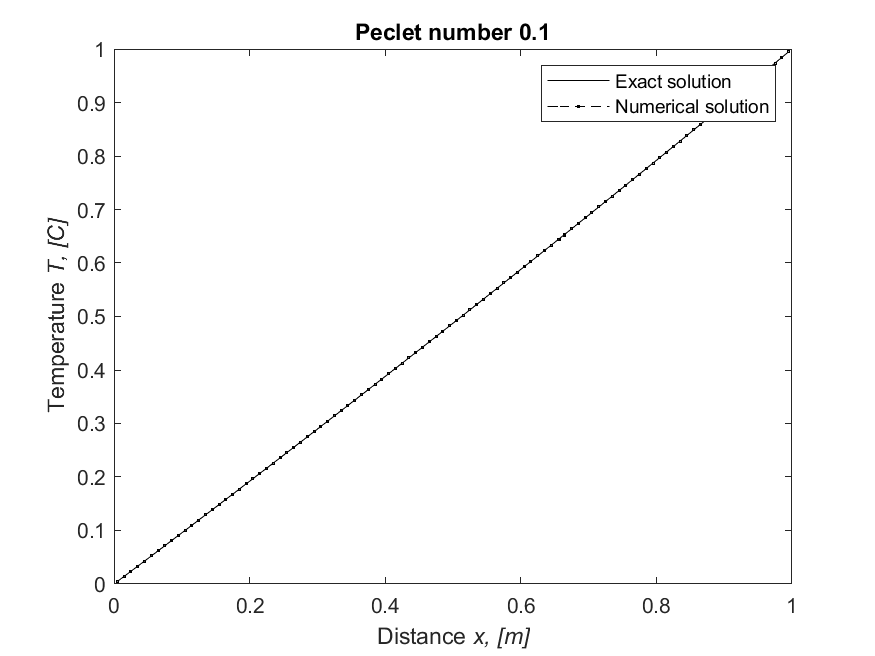
\includegraphics[width=\textwidth]{Questions/Code/peclet_0.1.png}
        \caption{Peclet number = 0.1}
    \end{subfigure}
    \begin{subfigure}{0.7\textwidth}
        \centering
        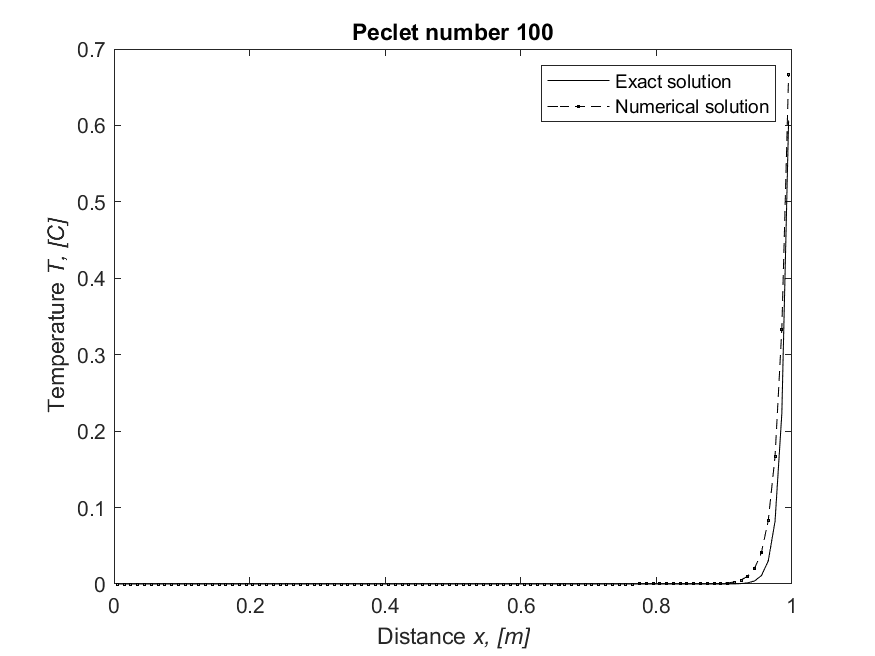
\includegraphics[width=\textwidth]{Questions/Code/peclet_100.png}
        \caption{Peclet number = 100}
    \end{subfigure}
    \caption{Analytical and numerical solutions for Peclet number = 0.1 and 100}
\end{figure}
\begin{figure}[H]
    \centering
    \begin{subfigure}{0.7\textwidth}
        \centering
        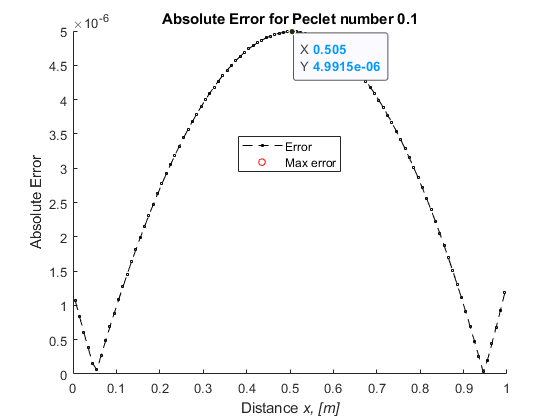
\includegraphics[width=\textwidth]{Questions/Code/error_0.1.png}
        \caption{Peclet number = 0.1}
    \end{subfigure}
    \begin{subfigure}{0.7\textwidth}
        \centering
        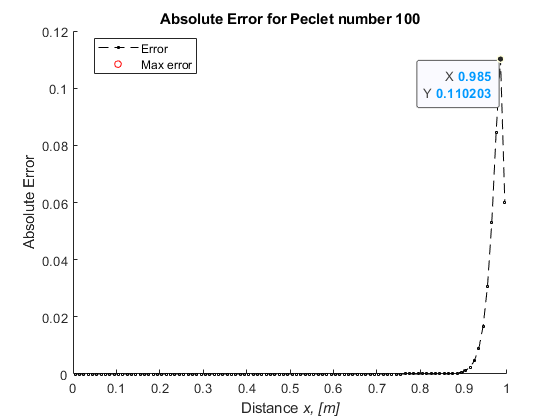
\includegraphics[width=\textwidth]{Questions/Code/error_100.png}
        \caption{Peclet number = 100}
    \end{subfigure}
    \caption{Absolute error for Peclet number = 0.1 and 100}
\end{figure}
% can you expand more on why small rate of diffusion leads to smooth temperature distribution and large rate of convection leads to steep temperature distribution?
Peclet number is the ratio between the rate of convection and the rate of diffusion. When the Peclet number is small, the rate of diffusion is much larger than the rate of convection. This means that the temperature distribution is dominated by the diffusion term. As a result, the temperature distribution is smooth and the temperature gradient is small. 

When the Peclet number is large, the rate of convection is much larger than the rate of diffusion. This means that the temperature distribution is dominated by the convection term. As a result, the temperature distribution is steep and the temperature gradient is large. 

The numerical solution is in good agreement with the analytical solution for both Peclet numbers. The maximum absolute error for Peclet number = 0.1 is $5$E-6 and the maximum absolute error for Peclet number = 100 is 0.11. 

A finer mesh is required to capture the steep temperature distribution for Peclet number = 100.\\

\lstinputlisting[language=Matlab]{Questions/Code/convdiff_CD.m}


% \newpage
% %\bibliographystyle{IEEEtran}
% %\bibliography{citations.bib}
% %\bibliography{}

% \newpage
% \appendix
% \section{Appendix: Arduino Uno Accuracy}
\label{sec:appendix-arduino-accuracy}
Table \ref{tab:arduino-accuracy-appendix} summarizes the range, resolution, repeatability, accuracy, and manufacturer's accuracy for various ranges of the 
Arduino Uno. Sample calculations for the 5V reference voltage are shown below. Note, the manufacturer's accuracy is $\pm$ 2 LSBs.

\begin{align*}
    \text{Resolution} &= \frac{V_{\text{ru}} - V_{\text{rl}}}{2^n} \\
    &= \frac{5.000 - 0.000}{2^{10}} \\
    &= \boxed{\qty[per-mode=symbol]{4.883}{\milli\volt\per\LSB}} \\
    \text{Repeatability} &= \max({\text{Max Deviation}}) \\
    &= \max(\langle 5.00, 0.00, 9.00, 44.00 \rangle) \\
    &= \boxed{\qty{44.00}{\milli\volt}} \\
    \text{Accuracy} &= \max({\text{Deviation}}) \\
    &= \max\left(
        \tiny	
        \begin{bmatrix}
            -0.009 & -0.009 & -0.009 & -0.009 & -0.009 & -0.009 & -0.009 & -0.009 & -0.004 & -0.009 \\
            0.001 & 0.001 & 0.001 & 0.001 & 0.001 & 0.001 & 0.001 & 0.001 & 0.001 & 0.001 \\
            0.016 & 0.021 & 0.012 & 0.016 & 0.012 & 0.012 & 0.016 & 0.016 & 0.012 & 0.016 \\
            0.02 & 0.024 & 0.02 & 0.024 & 0.01 & 0.02 & \textbf{0.054} & 0.024 & 0.034 & 0.02 \\
        \end{bmatrix}
    \right) \nonumber \\
    &= \boxed{\qty{54.00}{\milli\volt}}\\
    \text{Manuf. Acc.} &= \qty{2}{\LSB} \times \text{Resolution} \\
    &= \boxed{\qty{9.766}{\milli\volt}}
\end{align*}

\noindent For significant figures, since the range is given to 3 decimal places, the resolution is given to 3 decimal places, more often
than not, the number of significant figures is 4. This is because addition and subtraction do not take into account the number of significant figures
but rather the number of decimal places.

\begin{table}[ht]
    \caption{Range, Resolution, Repeatability, Accuracy, and Manufacturer's Accuracy for Various Ranges of the Arduino Uno}
    \label{tab:arduino-accuracy-appendix}
    \centering
    \small
    \begin{tabular}{lccccc}
        \toprule
        Arduino Config. & Range & Resolution & Repeatability & Acc. & Manuf. Acc. \\
        & (V) & (mV/LSB) & (mV) & (mV) & (mV) \\
        \midrule
        5V Ref. & 0.000 - 5.000 & 4.883 & 44.00 & 54.00 & 9.766 \\
        3.3V Ref. & 0.000 - 3.300 & 3.223 & 4.000 & 17.00 & 6.445 \\
        3.3V Ref., 10x VDiv & 0.00 - 33.00 & 32.23 & 32.00 & 83.00 & 64.45 \\
        3.3V Ref., [-10, 10]V & -10.00 - 10.00 & 19.53 & 0.000 & 24.00 & 39.06 \\
        3.3V Ref., 10x Amp. & 0.000 - 0.330 & 0.3223 & 0.000 & 0.000 & 0.6445 \\
        \bottomrule
    \end{tabular}
\end{table}

\FloatBarrier
\phantom{a}
\end{document}